\documentclass[a4paper,twocolumn,12pt]{article}
\usepackage[utf8]{inputenc}
\usepackage[MeX]{polski}
\usepackage{fullpage}
\usepackage{tikz}
\usetikzlibrary{calc,shapes,shapes.multipart, arrows}
\usepackage{pgfplots}
\pgfplotsset{compat=1.8}
\usepackage{hyperref}

% ;;;;;;;;; colors ;;;;;;;;;;;;

\definecolor{Board}{RGB}{60,145,143}
\definecolor{DoubleWordBonus}{RGB}{239,174,154}
\definecolor{DoubleLetterBonus}{RGB}{141,201,240}
\definecolor{TripleLetterBonus}{RGB}{54,156,219}
\definecolor{Tile}{RGB}{247,225,190}
\definecolor{UniGreen}{RGB}{0,100,200}

% ;;;;;;;;;;;;;;;;;;;;;;;;;;;;;;;;

\title{\LARGE{Sztuczna inteligencja grająca w~Scrabble} \\ \vspace{2mm} \large{Koncepcja implementacji - dane, struktury danych, algorytmy}}
\author{Jakub Turek}
\date{\today}

\begin{document}

\maketitle

\begin{abstract}
Celem artykułu jest opisanie zbioru koncepcji, które posłużą do implementacji algorytmu sztucznej inteligencji grającego w~grę Scrabble w~języku polskim. Artykuł analizuje i~porównuje dane zawarte w~dwóch głównych słownikach wyrazów do gier dla języka polskiego, przedstawia dane statystyczne ułatwiające wprowadzanie heurystyk do algorytmu, a~także opisuje metody niezbędne do wyznaczania wszystkich możliwych kombinacji ruchów w~danej turze. Autor omawia również podział rozgrywki na fazy gry i~przybliża podejście, które pozwala uzyskiwać najlepsze wyniki dla każdej fazy gry.
\end{abstract}

\section*{Wstęp}

Scrabble to ,,gra słowna polegająca na układaniu na określonej planszy wyrazów z~losowanych liter''\footnote{Wielki słownik ortograficzny - PWN 2003, 2006, 2008 - E. Polański}. Jest to bardzo ogólna definicja, którą należy uściślić. Scrabble jest grą przeznaczoną dla 2-4 osób. Akcesoriami do gry są: kwadratowa plansza o~stałym rozmiarze $15 \times 15$, torebka wypełniona płytkami, na których nadrukowane są litery oraz ich wartości punktowe, a~także stojaki, na których gracze umieszczają płytki, którymi w~danej chwili dysponują.

Gra rozgrywana jest w~turach. Zadaniem graczy jest układanie wyrazów na planszy, w~taki sposób aby tworzyły one poprawne słowa w~języku, w~którym prowadzona jest rozgrywka, w~układzie krzyżówkowym. Układ krzyżówkowy został przedstawiony na rysunkach \ref{fig:crossword_first} oraz \ref{fig:crossword_second}:

\begin{description}
 \item [Rysunek \ref{fig:crossword_first}] Pokazuje sytuację początkową obrazującą pewien moment rozgrywki.
 \item [Rysunek \ref{fig:crossword_second}] Pokazuje poprawny ruch zawodnika, który powoduje powstanie więcej niż jednego słowa. Wszystkie wyrazy utworzone przez jeden ruch muszą być poprawne. W~podanym przykładzie słowa ,,za'' i~,,masz'' są poprawne.
\end{description}

\begin{figure}[ht!]
	\begin{center}
			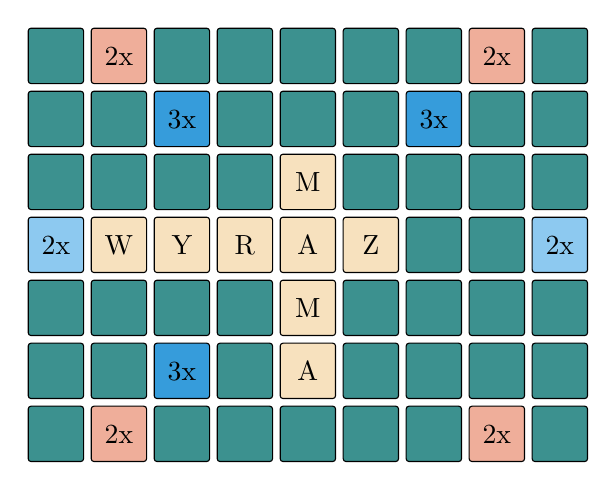
\begin{tikzpicture}
			\tikzstyle{every node}=[draw, shape=rectangle, rounded corners = 1pt, minimum width = 20pt, minimum height = 20pt, align=center, text height = 7pt];
			\node [fill=Board] at (-0.8, 0) {};
			\node [fill=DoubleWordBonus] at (0, 0) {2x};
			\node [fill=Board] at (0.8, 0) {};
			\node [fill=Board] at (1.6, 0) {};
			\node [fill=Board] at (2.4, 0) {};
			\node [fill=Board] at (3.2, 0) {};
			\node [fill=Board] at (4.0, 0) {};
			\node [fill=DoubleWordBonus] at (4.8, 0) {2x};
			\node [fill=Board] at (5.6, 0) {};
			\node [fill=Board] at (-.8, -.8) {};
			\node [fill=Board] at (0, -.8) {};
			\node [fill=TripleLetterBonus] at (0.8, -.8) {3x};
			\node [fill=Board] at (1.6, -.8) {};
			\node [fill=Board] at (2.4, -.8) {};
			\node [fill=Board] at (3.2, -.8) {};
			\node [fill=TripleLetterBonus] at (4.0, -.8) {3x};
			\node [fill=Board] at (4.8, -.8) {};
			\node [fill=Board] at (5.6, -.8) {};
			\node [fill=Board] at (-.8, -1.6) {};
			\node [fill=Board] at (0, -1.6) {};
			\node [fill=Board] at (0.8, -1.6) {};
			\node [fill=Board] at (1.6, -1.6) {};
			\node [fill=Tile] at (2.4, -1.6) {M};
			\node [fill=Board] at (3.2, -1.6) {};
			\node [fill=Board] at (4.0, -1.6) {};
			\node [fill=Board] at (4.8, -1.6) {};
			\node [fill=Board] at (5.6, -1.6) {};
			\node [fill=DoubleLetterBonus] at (-.8, -2.4) {2x};
			\node [fill=Tile] at (0, -2.4) {W};
			\node [fill=Tile] at (.8, -2.4) {Y};
			\node [fill=Tile] at (1.6, -2.4) {R};
			\node [fill=Tile] at (2.4, -2.4) {A};
			\node [fill=Tile] at (3.2, -2.4) {Z};
			\node [fill=Board] at (4.0, -2.4) {};
			\node [fill=Board] at (4.8, -2.4) {};
			\node [fill=DoubleLetterBonus] at (5.6, -2.4) {2x};
			\node [fill=Board] at (-.8, -3.2) {};
			\node [fill=Board] at (0, -3.2) {};
			\node [fill=Board] at (0.8, -3.2) {};
			\node [fill=Board] at (1.6, -3.2) {};
			\node [fill=Tile] at (2.4, -3.2) {M};
			\node [fill=Board] at (3.2, -3.2) {};
			\node [fill=Board] at (4.0, -3.2) {};
			\node [fill=Board] at (4.8, -3.2) {};
			\node [fill=Board] at (5.6, -3.2) {};
			\node [fill=Board] at (-.8, -4.0) {};
			\node [fill=Board] at (0, -4.0) {};
			\node [fill=TripleLetterBonus] at (0.8, -4.0) {3x};
			\node [fill=Board] at (1.6, -4.0) {};
			\node [fill=Tile] at (2.4, -4.0) {A};
			\node [fill=Board] at (3.2, -4.0) {};
			\node [fill=Board] at (4.0, -4.0) {};
			\node [fill=Board] at (4.8, -4.0) {};
			\node [fill=Board] at (5.6, -4.0) {};
			\node [fill=Board] at (-.8, -4.8) {};
			\node [fill=DoubleWordBonus] at (0, -4.8) {2x};
			\node [fill=Board] at (0.8, -4.8) {};
			\node [fill=Board] at (1.6, -4.8) {};
			\node [fill=Board] at (2.4, -4.8) {};
			\node [fill=Board] at (3.2, -4.8) {};
			\node [fill=Board] at (4.0, -4.8) {};
			\node [fill=DoubleWordBonus] at (4.8, -4.8) {2x};
			\node [fill=Board] at (5.6, -4.8) {};
		\end{tikzpicture}
		\caption{Fragment planszy. Gracze ułożyli kolejno słowa: ,,wyraz'' oraz ''mama''.}
		\label{fig:crossword_first}
	\end{center}
\end{figure}

\begin{figure}[ht!]
	\begin{center}
			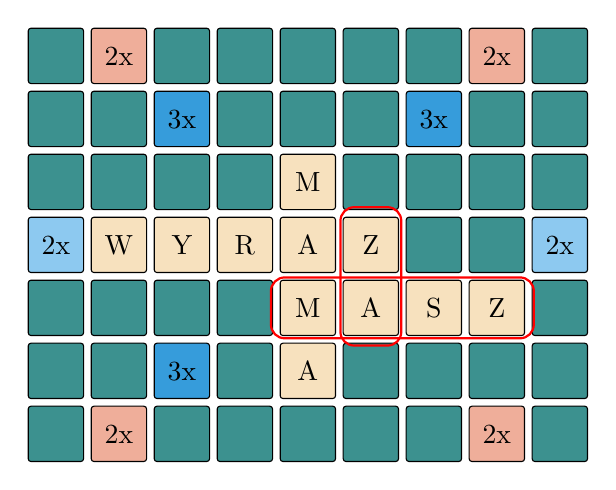
\begin{tikzpicture}
			\tikzstyle{every node}=[draw, shape=rectangle, rounded corners = 1pt, minimum width = 20pt, minimum height = 20pt, align=center, text height = 7pt];
			\node [fill=Board] at (-0.8, 0) {};
			\node [fill=DoubleWordBonus] at (0, 0) {2x};
			\node [fill=Board] at (0.8, 0) {};
			\node [fill=Board] at (1.6, 0) {};
			\node [fill=Board] at (2.4, 0) {};
			\node [fill=Board] at (3.2, 0) {};
			\node [fill=Board] at (4.0, 0) {};
			\node [fill=DoubleWordBonus] at (4.8, 0) {2x};
			\node [fill=Board] at (5.6, 0) {};
			\node [fill=Board] at (-.8, -.8) {};
			\node [fill=Board] at (0, -.8) {};
			\node [fill=TripleLetterBonus] at (0.8, -.8) {3x};
			\node [fill=Board] at (1.6, -.8) {};
			\node [fill=Board] at (2.4, -.8) {};
			\node [fill=Board] at (3.2, -.8) {};
			\node [fill=TripleLetterBonus] at (4.0, -.8) {3x};
			\node [fill=Board] at (4.8, -.8) {};
			\node [fill=Board] at (5.6, -.8) {};
			\node [fill=Board] at (-.8, -1.6) {};
			\node [fill=Board] at (0, -1.6) {};
			\node [fill=Board] at (0.8, -1.6) {};
			\node [fill=Board] at (1.6, -1.6) {};
			\node [fill=Tile] at (2.4, -1.6) {M};
			\node [fill=Board] at (3.2, -1.6) {};
			\node [fill=Board] at (4.0, -1.6) {};
			\node [fill=Board] at (4.8, -1.6) {};
			\node [fill=Board] at (5.6, -1.6) {};
			\node [fill=DoubleLetterBonus] at (-.8, -2.4) {2x};
			\node [fill=Tile] at (0, -2.4) {W};
			\node [fill=Tile] at (.8, -2.4) {Y};
			\node [fill=Tile] at (1.6, -2.4) {R};
			\node [fill=Tile] at (2.4, -2.4) {A};
			\node [fill=Tile] at (3.2, -2.4) {Z};
			\node [fill=Board] at (4.0, -2.4) {};
			\node [fill=Board] at (4.8, -2.4) {};
			\node [fill=DoubleLetterBonus] at (5.6, -2.4) {2x};
			\node [fill=Board] at (-.8, -3.2) {};
			\node [fill=Board] at (0, -3.2) {};
			\node [fill=Board] at (0.8, -3.2) {};
			\node [fill=Board] at (1.6, -3.2) {};
			\node [fill=Tile] at (2.4, -3.2) {M};
			\node [fill=Tile] at (3.2, -3.2) {A};
			\node [fill=Tile] at (4.0, -3.2) {S};
			\node [fill=Tile] at (4.8, -3.2) {Z};
			\node [fill=Board] at (5.6, -3.2) {};
			\node [fill=Board] at (-.8, -4.0) {};
			\node [fill=Board] at (0, -4.0) {};
			\node [fill=TripleLetterBonus] at (0.8, -4.0) {3x};
			\node [fill=Board] at (1.6, -4.0) {};
			\node [fill=Tile] at (2.4, -4.0) {A};
			\node [fill=Board] at (3.2, -4.0) {};
			\node [fill=Board] at (4.0, -4.0) {};
			\node [fill=Board] at (4.8, -4.0) {};
			\node [fill=Board] at (5.6, -4.0) {};
			\node [fill=Board] at (-.8, -4.8) {};
			\node [fill=DoubleWordBonus] at (0, -4.8) {2x};
			\node [fill=Board] at (0.8, -4.8) {};
			\node [fill=Board] at (1.6, -4.8) {};
			\node [fill=Board] at (2.4, -4.8) {};
			\node [fill=Board] at (3.2, -4.8) {};
			\node [fill=Board] at (4.0, -4.8) {};
			\node [fill=DoubleWordBonus] at (4.8, -4.8) {2x};
			\node [fill=Board] at (5.6, -4.8) {};
			\node [draw, thick, shape = rectangle, rounded corners = 5pt, color = red, fill = none, minimum height = 22 pt, minimum width = 95 pt] at (3.6, -3.2) {};
			\node [draw, thick, shape = rectangle, rounded corners = 5pt, color = red, fill = none, minimum width = 22 pt, minimum height = 50 pt] at (3.2, -2.8) {};
		\end{tikzpicture}
		\caption{Fragment planszy. Ruch przez dołożenie liter A, S, Z tworzy dwa wyrazy w~układzie krzyżówkowym.}
		\label{fig:crossword_second}
	\end{center}
\end{figure}

W~trakcie jednego ruchu zawodnik może układać płytki tylko w~jednym kierunku (pionowo lub poziomo). Utworzony przez zawodnika wyraz musi być spójny, to znaczy, że wszystkie płytki muszą przylegać do siebie bezpośrednio lub poprzez płytki już istniejące na planszy. Wymagane jest, aby tworzone słowo przylegało do przynajmniej jednej płytki, która jest już umieszczona na planszy (nie dotyczy to pierwszego ruchu).

Punktacja za dane zagranie jest obliczana jako suma punktów za wszystkie płytki, które wchodzą w~skład utworzonych wyrazów (a~więc również tych, które przed zagraniem znajdowały się na planszy), z~uwzględnieniem niewykorzystanych premii wynikających z~pozycji płytki na planszy:

\begin{description}
 \item [Premia literowa] Podwaja lub potraja wartość danej płytki.
 \item [Premia słowna] Podwaja lub potraja wartość całego wyrazu.
\end{description}

\section*{Słowniki do gier}

Reguły Scrabble dopuszczają układanie ,,wszystkich słów występujących w~słownikach języka polskiego oraz wszystkich ich prawidłowych form gramatycznych, z~wyjątkiem takich słów, które rozpoczynają się od wielkiej litery, są skrótami, bądź słowami wymagającymi cudzysłowu lub łącznika''\footnote{Reguły gry w~Scrabble z~witryny Polskiej Federacji Scrabble - \url{http://www.pfs.org.pl/zds.php}.}. 

Brak zamkniętej listy słów możliwych do wykorzystania w~grze prowadzi do konfliktu interesów, ponieważ gracze sami muszą rozstrzygnąć między sobą, czy dany wyraz jest legalny, bądź nie. Aby możliwa była uczciwa rozgrywka, konieczne było stworzenie słownika do gier. Słownik wyrazów do gier jest to lista wszystkich słów, wraz ze wszystkimi poprawnymi odmianami, dopuszczalnych do wykorzystania w~grach słownych\footnote{Anna Andrzejczuk, \emph{Słowniki do gier słownych jako nowy typ wydawnictw leksykograficznych}. Praca magisterska pod kierownictwem dr hab. R. Pawelec.}.

W~chwili obecnej istnieją dwa duże polskie słowniki do gier:

\begin{description}
 \item [Oficjalny Słownik Polskiego Scrabblisty] Przygotowany przez wydawnictwo naukowe PWN. Dopuszcza użycie wyrazów znajdujących się w~słownikach PWN wydanych po roku 1980.
 \item[Słownik alternatywny] Przygotowany na potrzeby serwisu z~grami przez Internet \url{http://kurnik.pl}. Jest rozwijany przez administratorów serwisu przy współpracy z~internautami. Dopuszcza użycie wyrazów znajdujących się w~słownikach dowolnego wydawnictwa wydanych po roku 1980, z~wyłączeniem czarnej listy słowników\footnote{Jest to lista słowników, które nie zostały dopuszczone jako źródło wyrazów ze względu na niedostateczną jakość opracowania.}. 
\end{description}

Poza dopuszczalnymi źródłami informacji, słowniki posiadają jeszcze jedną znaczącą różnicę. Oficjalny Słownik Polskiego Scrabblisty jest dystrybuowany jako program umieszczony na płycie CD, który nie udostępnia listy wszystkich wyrazów zawartych w~słowniku. Program pozwala wyłącznie sprawdzić, czy dane słowo jest legalne, bądź nie. Słownik alternatywny dostępny jest w Internecie również w~postaci listy wszystkich dopuszczalnych wyrazów zebranych w~pliku tekstowym. Pozwala to na przeprowadzenie analiz statystycznych. Stąd w~dalszej części artykułu autor rozważa wyłącznie Słownik alternatywny.

\section*{Analiza statystyczna}

W~celu wyznaczenia heurystyk mogących wspomóc sztuczną inteligencję grającą w~Scrabble, autor przeanalizował dane zawarte w~Słowniku alternatywnym. Pierwszą analizowaną informacją jest częstotliwość występowania poszczególnych liter w~słowniku. Wynika to z~faktu, że zasady gry Scrabble są oparte na rozkładzie prawdopodobieństwa występowania liter w~danym języku. Możliwe jest, że badanie statystyczne słownika przyniesie informacje o~literach, których warto używać w~pierwszej kolejności.

\begin{figure}[ht!]
	\begin{center}
		\begin{tikzpicture}
			\begin{axis}[	ytick={0, 0.01, ..., 0.1}, 
					yticklabel style={/pgf/number format/fixed},
					bar width=1mm,
					symbolic x coords={a,i,o,e,n,y,z,w,r,c,m,s,k,p,t,u,l,d,el,j,b,g,on,h,es,zet,een,f,uu,en,ci,ziet},
					xticklabels={a,i,o,e,n,y,z,w,r,c,m,s,k,p,t,u,l,d,ł,j,b,g,ą,h,ś,ż,ę,f,ó,ń,ć,ź},
					xticklabel style={font=\scriptsize, text height=1ex},
					xtick=data,
					yticklabel style={font=\scriptsize},
					legend entries={Prawdopodobieństwo dla słownika,Prawdopodobieństwo w Scrabble},
					legend style={font=\scriptsize},
					height=.3\textheight,
					width=.5\textwidth]
					
    			\addplot[ybar,fill=UniGreen, area legend] coordinates {
        			(a,0.0937997771175)
        			(i,0.0894002903657)
        			(o,0.0796720098207)
        			(e,0.0765123987403)
        			(n,0.0683027202572)
        			(y,0.0497071483395)
        			(z,0.0466694841626)
        			(w,0.0453746978807)
        			(r,0.0440417929225)
        			(c,0.0409715964269)
        			(m,0.0387468458849)
        			(s,0.0322800452968)
        			(k,0.0316402758911)
        			(p,0.029784849318)
        			(t,0.0273647734205)
        			(u,0.0271062565005)
        			(l,0.023888810187)
        			(d,0.0219487338635)
        			(el,0.0210803509823)
        			(j,0.0195483416618)
        			(b,0.0192369186479)
        			(g,0.0132131819509)
        			(on,0.0128586125387)
        			(h,0.0115084555932)
        			(es,0.0096922978289)
        			(zet,0.0064777761380)
        			(een,0.0064627258330)
        			(f,0.0044409243818)
        			(uu,0.0035346199898)
        			(en,0.0027972207673)
        			(ci, 0.0011952505312)
        			(ziet,0.0007161382021)
    			};
    			
    			\addplot[ybar,fill=lightgray, area legend] coordinates {
        			(a,0.09)
        			(i,0.08)
        			(o,0.06)
        			(e,0.07)
        			(n,0.05)
        			(y,0.04)
        			(z,0.05)
        			(w,0.04)
        			(r,0.04)
        			(c,0.03)
        			(m,0.03)
        			(s,0.04)
        			(k,0.03)
        			(p,0.03)
        			(t,0.03)
        			(u,0.02)
        			(l,0.03)
        			(d,0.03)
        			(el,0.02)
        			(j,0.02)
        			(b,0.02)
        			(g,0.02)
        			(on,0.01)
        			(h,0.02)
        			(es,0.01)
        			(zet,0.01)
        			(een,0.01)
        			(f,0.01)
        			(uu,0.01)
        			(en,0.01)
        			(ci, 0.01)
        			(ziet,0.01)
    			};
    			\addplot[forget plot,ybar,fill=UniGreen] coordinates {
        			(a,0)
        			(i,0)
        			(o,0)
        			(e,0)
        			(n,0)
        			(y,0)
        			(z,0.0466694841626)
        			(w,0)
        			(r,0)
        			(c,0)
        			(m,0)
        			(s,0.0322800452968)
        			(k,0)
        			(p,0.029784849318)
        			(t,0.0273647734205)
        			(u,0)
        			(l,0.023888810187)
        			(d,0.0219487338635)
        			(el,0)
        			(j,0.0195483416618)
        			(b,0.0192369186479)
        			(g,0.0132131819509)
        			(on,0)
        			(h,0.0115084555932)
        			(es,0.0096922978289)
        			(zet,0.0064777761380)
        			(een,0.0064627258330)
        			(f,0.0044409243818)
        			(uu,0.0035346199898)
        			(en,0.0027972207673)
        			(ci, 0.0011952505312)
        			(ziet,0.0007161382021)
    			};
			\end{axis}
		\end{tikzpicture}
		\caption{Wykres ilustrujący zależność pomiędzy wystąpieniem danej litery w~wyrazach słownika, a~prawdopodobieństwem wylosowania płytki z~tą literą w~grze Scrabble.}
		\label{fig:letter_probability_distribution}
	\end{center}
\end{figure}

Wykres przedstawiony na rysunku \ref{fig:letter_probability_distribution} dostarcza nam informacji, że autorzy polskich liter w~grze Scrabble nie oszacowali poprawnie częstotliwości występowania wszystkich liter. Przykładowo, wbrew zasadom gry, litera \textbf{o} w~rzeczywistości występuje częściej niż litera \textbf{e}. Wynika z~tego, że porównując dwa podobnie punktowane zagrania, warto wybrać to, które wykorzystuje więcej samogłosek \textbf{e} niż \textbf{o}. Podobną zależność można stwierdzić w~przypadku litery \textbf{h}, której częstotliwość występowania została przez autorów zasad znacząco zawyżona. Korzytnie jest wybierać zagrania, które powodują wyłożenie płytek z~literą \textbf{h}.

Interesującą statystyką są najlepsze otwarcia (czyli pierwsze zagrania w~grze). Pozwalają one, przy wylosowaniu szczęśliwej kombinacji płytek, zagrać w~najbardziej opłacalny sposób (na początku rozgrywki nie ma ryzyka pozostawienia przeciwnikowi ,,otwartej gry''). Statystyka ta jest szczególnie przydatna dla ludzi, chociaż również sztuczna inteligencja może wykorzystywać tego typu informacje do pominięcia zbędnych obliczeń. Najlepsze otwarcia dla słownika alternatywnego zebrano na rysunku \ref{fig:best_openings}.

\begin{figure}[ht!]
	\begin{center}
			\begin{tikzpicture}
		\tikzstyle{every node}=[draw, shape=rectangle, rounded corners = 1pt, minimum width = 16pt, minimum height = 16pt, align=center, text height = 5pt, font=\scriptsize];
		\node [fill=Board] at (0, 0) { };
		\node [fill=Board] at (.6, 0) { };
		\node [fill=DoubleLetterBonus] at (1.2, 0) {x2};
		\node [fill=Board] at (1.8, 0) { };
		\node [fill=Board] at (2.4, 0) { };
		\node [fill=Board] at (3, 0) { };
		\node [fill=DoubleWordBonus] at (3.6, 0) { };
		\node [fill=Board] at (4.2, 0) { };
		\node [fill=Board] at (4.8, 0) { };
		\node [fill=Board] at (5.4, 0) { };
		\node [fill=DoubleLetterBonus] at (6, 0) {x2};
		\node [fill=Board] at (6.6, 0) { };
		\node [fill=Board] at (7.2, 0) { };		
		\node [shape=star, star points=8, rounded corners = 0pt, fill=black, text height = 0pt] at (3.6, 0) {};
		\node [fill=Tile] at (0, -.6) {P};
		\node [fill=Tile] at (.6, -.6) {Ó};
		\node [fill=Tile] at (1.2, -.6) {Ź};
		\node [fill=Tile] at (1.8, -.6) {N};
		\node [fill=Tile] at (2.4, -.6) {O};
		\node [fill=Tile] at (3, -.6) {Ś};
		\node [fill=Tile] at (3.6, -.6) {Ć};
		\node [fill=Board] at (4.2, -.6) { };
		\node [fill=Board] at (4.8, -.6) { };
		\node [fill=Board] at (5.4, -.6) { };
		\node [fill=DoubleLetterBonus] at (6, -.6) {x2};
		\node [fill=Board] at (6.6, -.6) { };
		\node [fill=Board] at (7.2, -.6) { };	
		\node [fill=Board] at (0, -1.2) { };
		\node [fill=Board] at (.6, -1.2) { };
		\node [fill=DoubleLetterBonus] at (1.2, -1.2) {x2};
		\node [fill=Board] at (1.8, -1.2) { };
		\node [fill=Board] at (2.4, -1.2) { };
		\node [fill=Board] at (3, -1.2) { };
		\node [fill=Tile] at (3.6, -1.2) {B};
		\node [fill=Tile] at (4.2, -1.2) {Ł};
		\node [fill=Tile] at (4.8, -1.2) {Ą};
		\node [fill=Tile] at (5.4, -1.2) {D};
		\node [fill=Tile] at (6, -1.2) {Ź};
		\node [fill=Tile] at (6.6, -1.2) {Ż};
		\node [fill=Tile] at (7.2, -1.2) {E};
		\node [fill=Board] at (0, -1.8) { };
		\node [fill=Board] at (.6, -1.8) { };
		\node [fill=DoubleLetterBonus] at (1.2, -1.8) {x2};
		\node [fill=Board] at (1.8, -1.8) { };
		\node [fill=Board] at (2.4, -1.8) { };
		\node [fill=Board] at (3, -1.8) { };
		\node [fill=Tile] at (3.6, -1.8) {U};
		\node [fill=Tile] at (4.2, -1.8) {B};
		\node [fill=Tile] at (4.8, -1.8) {O};
		\node [fill=Tile] at (5.4, -1.8) {D};
		\node [fill=Tile] at (6, -1.8) {Ź};
		\node [fill=Tile] at (6.6, -1.8) {Ż};
		\node [fill=Tile] at (7.2, -1.8) {E};
		\node [fill=Board] at (0, -2.4) { };
		\node [fill=Board] at (.6, -2.4) { };
		\node [fill=DoubleLetterBonus] at (1.2, -2.4) {x2};
		\node [fill=Board] at (1.8, -2.4) { };
		\node [fill=Board] at (2.4, -2.4) { };
		\node [fill=Board] at (3, -2.4) { };
		\node [fill=Tile] at (3.6, -2.4) {P};
		\node [fill=Tile] at (4.2, -2.4) {Ó};
		\node [fill=Tile] at (4.8, -2.4) {J};
		\node [fill=Tile] at (5.4, -2.4) {D};
		\node [fill=Tile] at (6, -2.4) {Ź};
		\node [fill=Tile] at (6.6, -2.4) {K};
		\node [fill=Tile] at (7.2, -2.4) {Ę};		
		\node [fill=Board] at (0, -3) { };
		\node [fill=Board] at (.6, -3) { };
		\node [fill=DoubleLetterBonus] at (1.2, -3) {x2};
		\node [fill=Board] at (1.8, -3) { };
		\node [fill=Board] at (2.4, -3) { };
		\node [fill=Board] at (3, -3) { };
		\node [fill=Tile] at (3.6, -3) {G};
		\node [fill=Tile] at (4.2, -3) {Ł};
		\node [fill=Tile] at (4.8, -3) {Ó};
		\node [fill=Tile] at (5.4, -3) {D};
		\node [fill=Tile] at (6, -3) {Ź};
		\node [fill=Tile] at (6.6, -3) {Ż};
		\node [fill=Tile] at (7.2, -3) {E};	
		\node [fill=Board] at (0, -3.6) { };
		\node [fill=Board] at (.6, -3.6) { };
		\node [fill=DoubleLetterBonus] at (1.2, -3.6) {x2};
		\node [fill=Board] at (1.8, -3.6) { };
		\node [fill=Board] at (2.4, -3.6) { };
		\node [fill=Board] at (3, -3.6) { };
		\node [fill=Tile] at (3.6, -3.6) {U};
		\node [fill=Tile] at (4.2, -3.6) {B};
		\node [fill=Tile] at (4.8, -3.6) {Ą};
		\node [fill=Tile] at (5.4, -3.6) {D};
		\node [fill=Tile] at (6, -3.6) {Ź};
		\node [fill=Tile] at (6.6, -3.6) {Ż};
		\node [fill=Tile] at (7.2, -3.6) {E};		
		\node [fill=Board] at (0, -4.2) { };
		\node [fill=Board] at (.6, -4.2) { };
		\node [fill=DoubleLetterBonus] at (1.2, -4.2) {x2};
		\node [fill=Board] at (1.8, -4.2) { };
		\node [fill=Board] at (2.4, -4.2) { };
		\node [fill=Board] at (3, -4.2) { };
		\node [fill=Tile] at (3.6, -4.2) {U};
		\node [fill=Tile] at (4.2, -4.2) {G};
		\node [fill=Tile] at (4.8, -4.2) {Ó};
		\node [fill=Tile] at (5.4, -4.2) {D};
		\node [fill=Tile] at (6, -4.2) {Ź};
		\node [fill=Tile] at (6.6, -4.2) {Ż};
		\node [fill=Tile] at (7.2, -4.2) {E};		
		\node [fill=Board] at (0, -4.8) { };
		\node [fill=Board] at (.6, -4.8) { };
		\node [fill=DoubleLetterBonus] at (1.2, -4.8) {x2};
		\node [fill=Board] at (1.8, -4.8) { };
		\node [fill=Board] at (2.4, -4.8) { };
		\node [fill=Board] at (3, -4.8) { };
		\node [fill=Tile] at (3.6, -4.8) {B};
		\node [fill=Tile] at (4.2, -4.8) {L};
		\node [fill=Tile] at (4.8, -4.8) {U};
		\node [fill=Tile] at (5.4, -4.8) {Ź};
		\node [fill=Tile] at (6, -4.8) {Ń};
		\node [fill=Tile] at (6.6, -4.8) {Ż};
		\node [fill=Tile] at (7.2, -4.8) {E};	
		\node [fill=Board] at (0, -5.4) { };
		\node [fill=Board] at (.6, -5.4) { };
		\node [fill=DoubleLetterBonus] at (1.2, -5.4) {x2};
		\node [fill=Board] at (1.8, -5.4) { };
		\node [fill=Board] at (2.4, -5.4) { };
		\node [fill=Board] at (3, -5.4) { };
		\node [fill=Tile] at (3.6, -5.4) {P};
		\node [fill=Tile] at (4.2, -5.4) {Ó};
		\node [fill=Tile] at (4.8, -5.4) {J};
		\node [fill=Tile] at (5.4, -5.4) {D};
		\node [fill=Tile] at (6, -5.4) {Ź};
		\node [fill=Tile] at (6.6, -5.4) {K};
		\node [fill=Tile] at (7.2, -5.4) {Ą};		
		\node [fill=Board] at (0, -6) { };
		\node [fill=Board] at (.6, -6) { };
		\node [fill=DoubleLetterBonus] at (1.2, -6) {x2};
		\node [fill=Board] at (1.8, -6) { };
		\node [fill=Board] at (2.4, -6) { };
		\node [fill=Tile] at (3, -6) {U};
		\node [fill=Tile] at (3.6, -6) {G};
		\node [fill=Tile] at (4.2, -6) {R};
		\node [fill=Tile] at (4.8, -6) {Z};
		\node [fill=Tile] at (5.4, -6) {Ą};
		\node [fill=Tile] at (6, -6) {Ź};
		\node [fill=Tile] at (6.6, -6) {Ć};
		\node [fill=Board] at (7.2, -6) { };		
	\end{tikzpicture}
	\caption{Najlepsze otwarcia dla Słownika alternatywnego. Słowo \emph{późność} jest warte 126 punktów, pozostałe po 124 punkty.}
	\label{fig:best_openings}
	\end{center}
\end{figure}

Dokonując statycznej analizy słownika, warto wziąć pod uwagę najbardziej opłacalne kombinacje liter. W~trakcie rozgrywki gracze dążą do układania wyrazów, które wymagają użycia wszystkich siedmiu płytek znajdujących się na stojaku. Zagranie takie jest bowiem punktowane dodatkową premią w~wysokości 50 punktów. Stąd przez najbardziej opłacalną kombinację liter należy rozumieć taką zawartość stojaka, która pozwala ułożyć jak najwięcej wyrazów siedmioliterowych. Duża liczba kombinacji powoduje, że ułożony wyraz uda się wpasować w~istniejące na planszy ułożenie płytek z~większym prawdopodobieństwem. Autor przeanalizował najlepsze kombinacje liter dla Słownika alternatywnego. Wyniki zebrane są w~tabeli \ref{tab:best_letter_combos}.

\begin{figure}[ht!]
	\begin{center}
				\scalebox{0.9}{
				\begin{tabular}{|c|c|}
					\hline
					Litery	&	Liczba możliwych do	 \\
					& ułożenia wyrazów \\
					\hline
					E, I, K, L, N, O, W	&	12 słów	\\
					A, E, I, K, P, R, S	&	12 słów	\\
					A, E, I, K, L, N, P	&	12 słów	\\
					A, E, K, N, R, T, Y	&	11 słów	\\
					A, I, K, M, O, P, S&	11 słów	\\
					A, I, K, M, O, R, W&	11 słów	\\
					A, A, I, K, L, M, S	&	10 słów	\\
					A, I, K, M, O, S, T&	10 słów	\\
					A, I, K, L, N, O, W	&	10 słów	\\
					A, I, K, L, M, N, O&	10 słów	\\
					\hline
				\end{tabular}
				}
			\caption{Najlepsze kombinacje liter dla Słownika alternatywnego.}
			\label{tab:best_letter_combos}
	\end{center}
\end{figure}

Najbardziej opłacalne kombinacje liter można wykorzystać do strategicznego planowania zagrań. Wykonując poszczególne ruchy korzystnie jest dążyć do uzyskania jednego z~przedstawionych układów liter na stojaku. Można tego dokonać poprzez usuwanie płytek, które nie zostały uwzględnione w~tych kombinacjach, jak również usuwanie płytek zduplikowanych (częstą sytuacją jest posiadanie kilku płytek z~tą samą samogłoską).

\section*{Wyznaczanie wszystkich legalnych ruchów}

Podstawowym zadaniem sztucznej inteligencji w~grze Scrabble jest wyznaczenie wszystkich kombinacji ruchów w~danej turze, na podstawie zadanego słownika. Odpowiedni algorytm został opracowany przez A.~Appela i~G.~Jacobsona\footnote{,,The world's fastest Scrabble program'', {\em Communications of the ACM}, 31(5):572--585, 1988.}. Autorzy proponują opisanie słownika za pomocą grafowej stuktury o~nazwie DAWG\footnote{Z~angielskiego Directed Acyclic Word Graph - skierowany, niecykliczny graf słów.}. Jest to odmiana drzewa trie\footnote{Od angielskiego słowa \emph{retrieval}, które oznacza odczyt.}, która charakteryzuje się silną kompresją danych uzyskiwaną dzięki łączeniu krawędziami identycznych sufiksów wyrazów. Przykładowy słownik DAWG został przedstawiony na rysunku \ref{fig:dawg_example}.

\begin{figure}[ht!]
	\begin{center}
			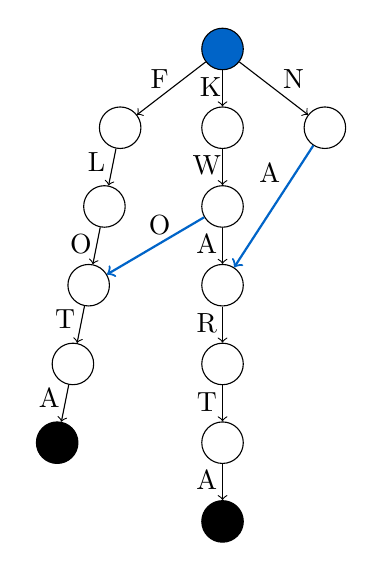
\begin{tikzpicture}
				\tikzstyle{every node}=[draw, shape=circle, minimum width = 15pt, minimum height = 15pt, text height = 0pt];
				\node [fill=UniGreen] (root) at (0,0) {};
				\node (n01) at (-1.3,-1) {};
				\node (n02) at (0, -1) {};
				\node (n03) at (1.3, -1) {};
				\node [draw=none] (t01) at (-0.8, -0.5) {F};
				\node [draw=none] (t02) at (-0.15, -0.6) {K};
				\node [draw=none] (t01) at (0.9, -0.5) {N};
				\draw[->] (root) -- (n01);
				\draw[->] (root) -- (n02);
				\draw[->] (root) -- (n03);
				\node (n11) at (-1.5, -2) {};
				\node (n12) at (0, -2) {};
				\node [draw=none] (t11) at (-1.6, -1.55) {L};
				\node [draw=none] (t12) at (-0.2, -1.6) {W};
				\node [draw=none] (t23) at (0.6, -1.7) {A};
				\draw[->] (n01) -- (n11);
				\draw[->] (n02) -- (n12);
				\node (n21) at (-1.7, -3) {};
				\node (n22) at (0, -3) {};
				\node [draw=none] (t21) at (-1.8, -2.6) {O};
				\node [draw=none] (t22) at (-0.8, -2.35) {O};
				\node [draw=none] (t23) at (-0.2, -2.6) {A};
				\draw[->] (n11) -- (n21);
				\draw[->, color=UniGreen, thick] (n12) -- (n21);
				\draw[->] (n12) -- (n22);
				\draw[->, color=UniGreen, thick] (n03) -- (n22);
				\node (n31) at (-1.9, -4) {};
				\node (n32) at (0, -4) {};
				\node [draw=none] (t31) at (-2.0, -3.55) {T};
				\node [draw=none] (t32) at (-0.2, -3.6) {R};
				\draw[->] (n21) -- (n31);
				\draw[->] (n22) -- (n32);
				\node [fill=black] (n41) at (-2.1, -5) {};
				\node (n42) at (0, -5) {};
				\node [draw=none] (t41) at (-2.2, -4.55) {A};
				\node [draw=none] (t42) at (-0.2, -4.6) {T};
				\draw[->] (n31) -- (n41);
				\draw[->] (n32) -- (n42);
				\node [fill=black] (n51) at (0, -6) {};
				\node [draw=none] (t51) at (-0.2, -5.6) {A};
				\draw[->] (n42) -- (n51);
			\end{tikzpicture}
			\caption{Struktura DAWG, która opisuje wyrazy flota, kwota, kwarta oraz narta.}
			\label{fig:dawg_example}
	\end{center}
\end{figure}

Autorzy wybrali tę strukturę ze względu na bardzo szybkie przeszukiwanie słów po ich prefiksie, a~także na dobry współczynnik kompresji słownika. Pełen słownik do gier dla języka angielskiego opisany przy pomocy DAWG zajmuje około $2.5$ MB pamięci.

Korzystając ze słownika DAWG, autorzy przedstawili czterokrokowy algorytm (zwany dalej algorytmem Appela-Jacobsona), który umożliwia wyznaczenie wszystkich możliwych ruchów przy danym stanie planszy i~określonych dostępnych do wykorzystania literach:

\begin{enumerate}
 \item Redukcja złożoności problemu do jednego wymiaru. Algorytm rozpatruje ruchy wyłącznie w~jednym kierunku (pionowo lub poziomo), ograniczając się do jednego wiersza lub kolumny. Rozumowanie to jest powtarzane dla każdego wiersza (lub kolumny), a~następnie plansza do gry jest transponowana i~algorytm wykonywany jest dla drugiego kierunku. W~dalszym opisie autor artykułu zakłada, że rozpatrujemy wyłącznie wiersze, a~nie kolumny, planszy.
 \item Ograniczanie zbioru znaków, które można legalnie wstawić w~daną komórkę. W~tym kroku wykorzystuje się fakt, że tworzenie wyrazów w~danym kierunku może skutkować utworzeniem nowych słów w~kierunku przeciwnym, ale tylko poprzez dodanie jednego znaku. Jest to trywialny do sprawdzenia przypadek, który znacząco ogranicza liczbę możliwych do wykonania legalnych ruchów.
 \item Wyznaczenie kotwic\footnote{W~oryginalnej pracy termin ten został wprowadzony przy pomocy angielskiego zwrotu \emph{anchor}.}. Kotwica jest to najbardziej wysunięta na lewo płytka nowego wyrazu, która przylega do innej, znajdującej się na planszy płytki. Zgodnie z~zasadami gry w~Scrabble, każdy nowo utworzony wyraz musi posiadać dokładnie jedną kotwicę.
 \item Rozwijanie możliwych do utworzenia wyrazów, poprzez wyjście od wyznaczonych w~punkcie trzecim kotwic, a~także uwzględnienie wyznaczonych w~punkcie drugim ograniczeń. 
\end{enumerate}

Rozwijanie możliwych wyrazów rozpoczyna się od płytek znajdujących się po lewej stronie kotwicy. Rozpatrywane są trzy przypadki:

\begin{itemize}
 \item Trywialny - na lewo od kotwicy nie ma żadnych płytek.
 \item Trywialny - część wyrazu na lewo od kotwicy składa się wyłącznie z~płytek znajdujących się już na planszy.
 \item Lewa część wyrazu składa się z~liter znajdujących się na stojaku i~dostępnych do zagrania. Należy zbadać wszystkie możliwe kombinacje.
\end{itemize}

Następnie rozwijana jest prawa część wyrazu, która uwzględnia kotwicę oraz wszystkie płytki na prawo od niej. W~tym celu wyszukuje się w~słowniku poprawne sufiksy, które składają się z~dostępnych na stojaku liter oraz spełniają wyznaczone ograniczenia.

Algorytm Appela-Jacobsona jest wydajny, jednak posiada narzut obliczeniowy związany z~wyznaczaniem lewostronnych dopełnień wyrazów. Zakładając, że kotwica jest również ostatnią literą nowego wyrazu, należy zbadać $6! = 720$ lewostronnych kombinacji. W~pesymistycznym przypadku, kiedy na stojaku znajdują się dwa blanki\footnote{Blank - płytka, która nie posiada wartości punktowej, ale może być zastąpiona dowolną literą.}, liczba badanych kombinacji wzrasta do $\frac{4! \times 32^{2}}{2} = 12288$, co jest znaczącym narzutem, biorąc pod uwagę fakt, że większość wyznaczonych prefiksów w~ogóle nie będzie występować w~słowniku.

Powyższa obserwacja stała się podstawą zmodyfikowanego algorytmu, zaprezentowanego przez Stevena Gordona\footnote{A Faster Scrabble Move Generation Algorithm, \em{Software - Practice and Experience}, 24(2):219--232, 1994.}. Autor nie zmienia kroków algorytmu wykorzystywanych do generacji wszystkich kombinacji ruchów. Zaproponowana modyfikacja obejmuje wykorzystanie struktury GADDAG\footnote{Autor nie podaje rozwinięcia tego skrótu, jednak ze względu na postać przechowywanych w~strukturze danych, można domyślać się, że jest ona wariacją nazwy DAG (z~angielskiego Directed Acyclic Graph - skierowany, acykliczny graf).}, w~miejsce słownika DAWG. 

GADDAG jest wariacją drzewa trie, która jest nastawiona na szybkie prefiksowanie wyrazów. Każdy opisany wyraz podzielony jest na dwie części - prefiks oraz sufiks. Wychodząc od korzenia drzewa, kolejne wierzchołki opisują prefiks wyrazu czytany od tyłu. Następnie występuje znak zakończenia prefiksu (oznaczany $\gg$), a~później sufiks wyrazu czytany w~normalnej kolejności. Kształt struktury jest silnie powiązany z~algorytmem Appela-Jacobsona. Wychodząc od kotwicy w~lewą stronę wyrazu, napotykamy kolejne litery prefiksu w~odwróconej kolejności. Następnie przechodzimy do kotwicy i~analizujemy sufiks w~normalnej kolejności. Ilustruje to rysunek \ref{fig:gaddag_basis}. 

\begin{figure}[ht!]
	\begin{center}
			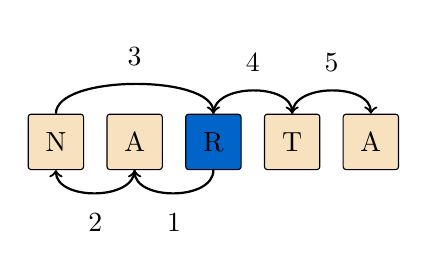
\begin{tikzpicture}
			\tikzstyle{every node}=[draw, shape=rectangle, rounded corners = 1pt, minimum width = 20pt, minimum height = 20pt, align=center, text height = 7pt];
			\node [fill=Tile] (n) at (0, 0) {N};
			\node [fill=Tile] (a1) at (1.0, 0) {A};
			\node [fill=UniGreen] (r) at (2.0, 0) {R};
			\node [fill=Tile] (t) at (3.0, 0) {T};
			\node [fill=Tile] (a2) at (4.0, 0) {A};
			\path (r) edge[out=270,in=270,->, thick] node[below, draw=none, fill=none]{$1$} (a1);
			\draw (a1) edge[out=270,in=270,->, thick] node[below, draw=none, fill=none]{$2$} (n);
			\draw (n) edge[out=90,in=90,->, thick, distance=0.5cm] node[above, draw=none, fill=none]{$3$} (r);
			\draw (r) edge[out=90,in=90,->, thick] node[above, draw=none, fill=none]{$4$} (t);
			\draw (t) edge[out=90,in=90,->, thick] node[above, draw=none, fill=none]{$5$} (a2);
		\end{tikzpicture}
	\end{center}
	\caption{Kolejność analizowania pól w~algorytmie Appela-Jacobsona. Kotwica oznaczona jest na niebiesko.}
	\label{fig:gaddag_basis}
\end{figure}

Przykładowa struktura GADDAG opisująca wyraz narta została zaprezentowana na rysunku \ref{fig:gaddag_example}. Należy zauważyć, że sprawdzenie występowania wyrazu w~słowniku wymaga dodatkowego kroku - należy go odwrócić. Dla podanego przykładu, sprawdzenie legalności wyrazu narta wymaga poszukiwania frazy $ATRAN \gg$. 

\begin{figure}[ht!]
	\begin{center}
	\scalebox{0.85}{
			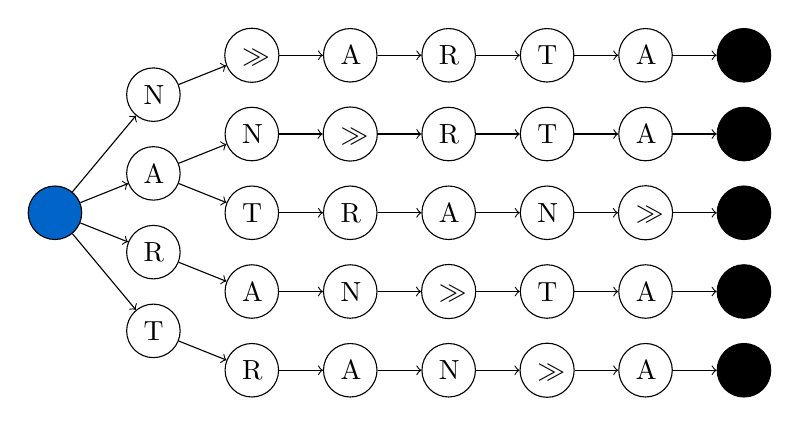
\begin{tikzpicture}
		\tikzstyle{every node}=[draw, shape=circle, minimum width = 15pt, minimum height = 15pt, text height = 7pt, text width = 7pt, align = center];
		\node [fill=UniGreen] (root) at (0,0) {};
		\node (n01) at (1.25, 1.5) {N};
		\node (n02) at (1.25, 0.5) {A};
		\node (n03) at (1.25, -0.5) {R};
		\node (n04) at (1.25, -1.5) {T};
		\node (n11) at (2.5, 2) {$\gg$};
		\node (n12) at (2.5, 1) {N};
		\node (n13) at (2.5, 0) {T};
		\node (n14) at (2.5, -1) {A};
		\node (n15) at (2.5, -2) {R};
		\node (n21) at (3.75, 2) {A};
		\node (n22) at (3.75, 1) {$\gg$};
		\node (n23) at (3.75, 0) {R};
		\node (n24) at (3.75, -1) {N};
		\node (n25) at (3.75, -2) {A};
		\node (n31) at (5, 2) {R};
		\node (n32) at (5, 1) {R};
		\node (n33) at (5, 0) {A};
		\node (n34) at (5, -1) {$\gg$};
		\node (n35) at (5, -2) {N};
		\node (n41) at (6.25, 2) {T};
		\node (n42) at (6.25, 1) {T};
		\node (n43) at (6.25, 0) {N};
		\node (n44) at (6.25, -1) {T};
		\node (n45) at (6.25, -2) {$\gg$};
		\node (n51) at (7.5, 2) {A};
		\node (n52) at (7.5, 1) {A};
		\node (n53) at (7.5, 0) {$\gg$};
		\node (n54) at (7.5, -1) {A};
		\node (n55) at (7.5, -2) {A};
		\node [fill=black] (n61) at (8.75, 2) {};
		\node [fill=black] (n62) at (8.75, 1) {};
		\node [fill=black] (n63) at (8.75, 0) {};
		\node [fill=black] (n64) at (8.75, -1) {};
		\node [fill=black] (n65) at (8.75, -2) {};
		\draw[->] (root) -- (n01);
		\draw[->] (root) -- (n02);
		\draw[->] (root) -- (n03);
		\draw[->] (root) -- (n04);
		\draw[->] (n01) -- (n11);
		\draw[->] (n02) -- (n12);
		\draw[->] (n02) -- (n13);
		\draw[->] (n03) -- (n14);
		\draw[->] (n04) -- (n15);
		\draw[->] (n11) -- (n21);
		\draw[->] (n12) -- (n22);
		\draw[->] (n13) -- (n23);
		\draw[->] (n14) -- (n24);
		\draw[->] (n15) -- (n25);
		\draw[->] (n21) -- (n31);
		\draw[->] (n22) -- (n32);
		\draw[->] (n23) -- (n33);
		\draw[->] (n24) -- (n34);
		\draw[->] (n25) -- (n35);
		\draw[->] (n31) -- (n41);
		\draw[->] (n32) -- (n42);
		\draw[->] (n33) -- (n43);
		\draw[->] (n34) -- (n44);
		\draw[->] (n35) -- (n45);
		\draw[->] (n41) -- (n51);
		\draw[->] (n42) -- (n52);
		\draw[->] (n43) -- (n53);
		\draw[->] (n44) -- (n54);
		\draw[->] (n45) -- (n55);
		\draw[->] (n51) -- (n61);
		\draw[->] (n52) -- (n62);
		\draw[->] (n53) -- (n63);
		\draw[->] (n54) -- (n64);
		\draw[->] (n55) -- (n65);
	\end{tikzpicture}
	}
		\caption{Przykład struktury GADDAG dla wyrazu narta.}
		\label{fig:gaddag_example}
	\end{center}
\end{figure}

\section*{Dobór strategii w~zależności od fazy gry}

Rozgrywkę w~Scrabble można podzielić na trzy fazy gry:

\begin{description}
 \item [MG (mid-game)] trwa od rozpoczęcia rozgrywki, do rozpoczęcia fazy \emph{PEG},
 \item [PEG (pre-endgame)] rozpoczyna się, kiedy do pobrania pozostają wyłącznie jedna (lub, w~zależności od definicji) dwie płytki,
 \item [EG (end-game)] rozpoczyna się, kiedy nie ma już płytek do pobrania, a~więc gracze znają wzajemnie własne płytki.
\end{description}

W~fazie \emph{MG} liczba możliwych kombinacji płytek przeciwnika oraz ruchów jest tak duża, że nie jest możliwa analiza przestrzeni stanów. Podejściem stosowanym w~tej fazie rozgrywki jest wykorzystanie metod heurystycznych i~symulacji do wyboru najlepszego ruchu. Schemat postępowania zostanie opisany na przykładzie algorytmu wykorzystywanego w~programie \emph{Quackle}\footnote{\url{http://people.csail.mit.edu/jasonkb/quackle/doc/how_quackle_plays_scrabble.html}} - uznawanym za najlepszego komputerowego gracza Scrabble na świecie. Diagram ilustrujący algorytm został przedstawiony na rysunku \ref{fig:quackle_schema}.

\begin{figure}[ht!]
 	\begin{center}
		\scalebox{0.63}{
			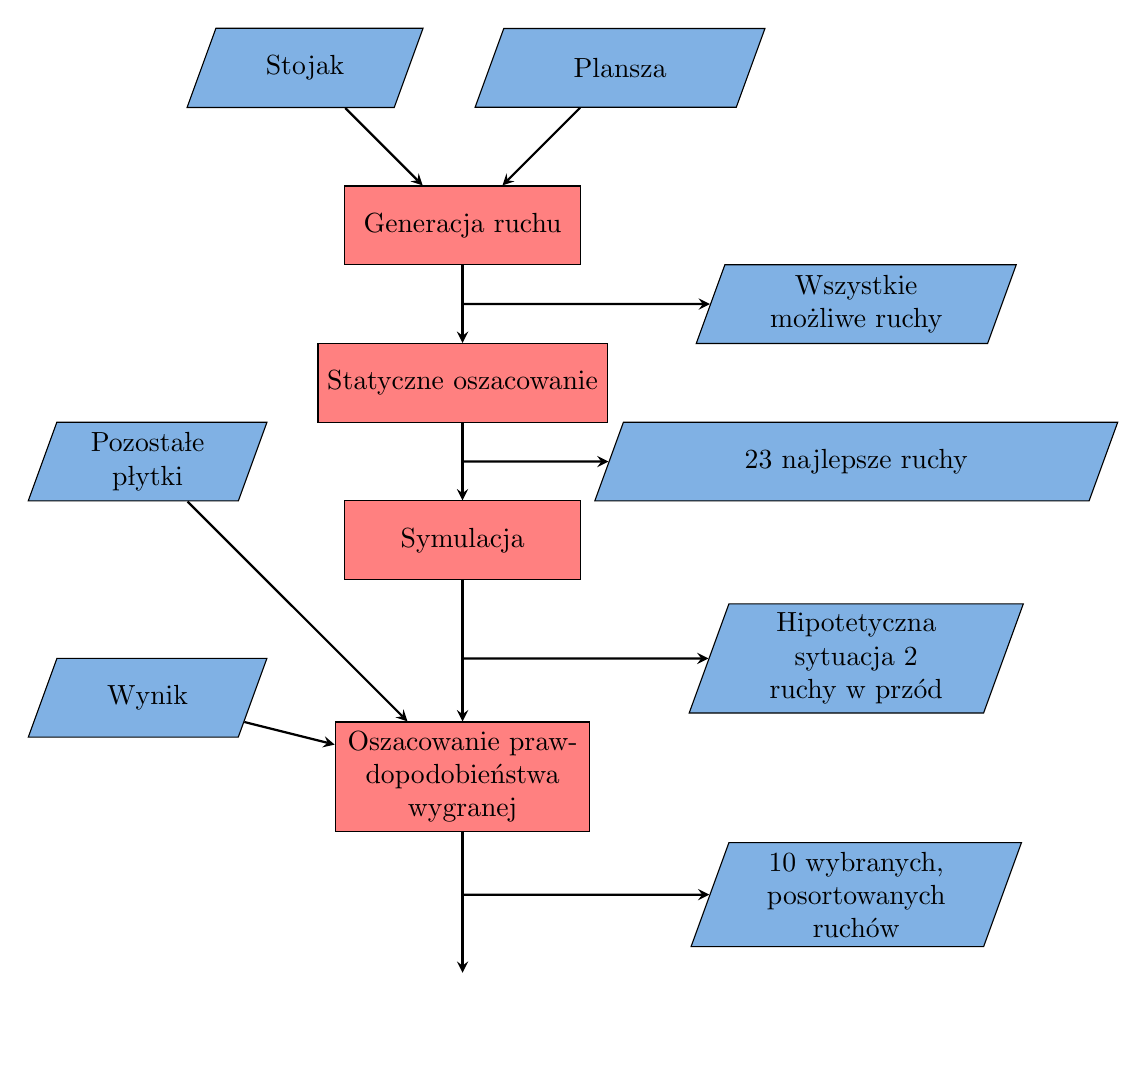
\begin{tikzpicture}[node distance=2cm]
				\tikzstyle{io} = [trapezium, trapezium left angle=70, trapezium right angle=110, minimum width=3cm, minimum height=1cm, text centered, draw=black, fill=UniGreen!50]
				\tikzstyle{process} = [rectangle, minimum width=3cm, minimum height=1cm, text centered, draw=black, fill=red!50]
				\tikzstyle{arrow} = [thick,->,>=stealth]
				
				\node (rack) [io] {Stojak};
				\node (board) [io, right of=rack, xshift=2cm] {Plansza};
				\coordinate (rackboard) at ($(rack)!0.5!(board)$);
				\node (movegen) [process, below of= rackboard] {Generacja ruchu};
				\node (staticeval) [process, below of=movegen] {Statyczne oszacowanie};
				\coordinate (movegenstaticeval) at ($(movegen)!0.5!(staticeval)$);
				\node (possmoves) [io, right of=movegenstaticeval, xshift=3cm, text width=3cm] {Wszystkie możliwe ruchy};
				\node (simulation) [process, below of=staticeval] {Symulacja};
				\node (bestmoves) [io, below of=possmoves, text width=3cm] {23 najlepsze ruchy};
				\node (hypsequences) [io, below of=bestmoves, text width=3cm, yshift=-0.5cm] {Hipotetyczna sytuacja 2 ruchy w~przód};
				\node (winpercestimation) [process, below of=simulation, text width=3cm, yshift=-1cm] {Oszacowanie prawdopodobieństwa wygranej};
				\node (end) [process, draw=none, fill=none, below of=winpercestimation, yshift=-1cm] { };
				\coordinate (staticevalsimulation) at ($(staticeval)!0.5!(simulation)$);
				\node (tilesleft) [io, left of=staticevalsimulation,xshift=-2cm, text width=2cm] {Pozostałe płytki};
				\node (score) [io, below of=tilesleft, yshift=-1cm] {Wynik};
				\coordinate (winpercestimationend) at ($(winpercestimation)!0.5!(end)$);
				\node (chosenmoves) [io, below of=hypsequences,text width=3cm, yshift=-1cm] {10 wybranych, posortowanych ruchów};
				\draw [arrow] (movegen) -- (staticeval);
				\draw [arrow] (staticeval) -- (simulation);
				\draw [arrow] (simulation) -- (winpercestimation);
				\draw [arrow] (rack) -- (movegen);
				\draw [arrow] (board) -- (movegen);
				\draw [arrow] (winpercestimation) -- (end);
				\draw [arrow] (tilesleft) -- (winpercestimation);
				\draw [arrow] (score) -- (winpercestimation);
				\draw [arrow] ($(movegen)!0.5!(staticeval)$) -- (possmoves);
				\draw [arrow] ($(staticeval)!0.5!(simulation)$) -- (bestmoves);
				\draw [arrow] ($(simulation)!0.5!(winpercestimation)$) -- (hypsequences);
				\draw [arrow] ($(winpercestimation)!0.5!(end)$) -- (chosenmoves);
			\end{tikzpicture}
			}
			\caption{Schemat blokowy algorytmu wykorzystywanego w~aplikacji \emph{Quackle}.}
			\label{fig:quackle_schema}
	\end{center}
\end{figure}

\emph{Quackle} wykorzystuje następujący algorytm:

\begin{enumerate}
 \item Generacja wszystkich dopuszczalnych możliwości ruchu.
 \item Przypisanie każdej z~możliwości statycznego oszacowania. Funkcja wykorzystywana do szacowania może być tak prosta, jak suma punktów uzyskanych za dane zagranie.
 \item Sortowanie ruchów od najlepszego do najgorszego względem statycznego oszacowania.
 \item Wylosowanie prawdopodobnego układu płytek, którymi może dysponować przeciwnik.
 \item Symulacja przeprowadzana dla 23 najlepszych ruchów. Dla wylosowanego układu płytek przeciwnika symulowana jest partia na dwa kroki w~przód. Do oceny wykorzystuje się wynik punktowy po przeprowadzeniu symulacji.
 \item Na podstawie wyniku rozgrywki i~liczby płytek pozostałych do pobrania szacowane jest prawdopodobieństwo wygranej dla każdego z~zasymulowanych ruchów.
 \item Wybieranych jest 10 ruchów dających największe prawdopodobieństwo wygranej.
 \item Na podstawie dodatkowych czynników (przykładowo: zestawu wykorzystanych w~danym ruchu liter) wybierana jest najlepsza możliwość.
\end{enumerate}


\end{document}
